% File: algo.tex
% Date: Thu Jun 20 17:49:43 2013 +0800
% Author: Yuxin Wu <ppwwyyxxc@gmail.com>
\section{算法说明}
\subsection{光线追踪}
光线追踪的基本原理如下图所示.
\begin{figure}[H]
  \centering
  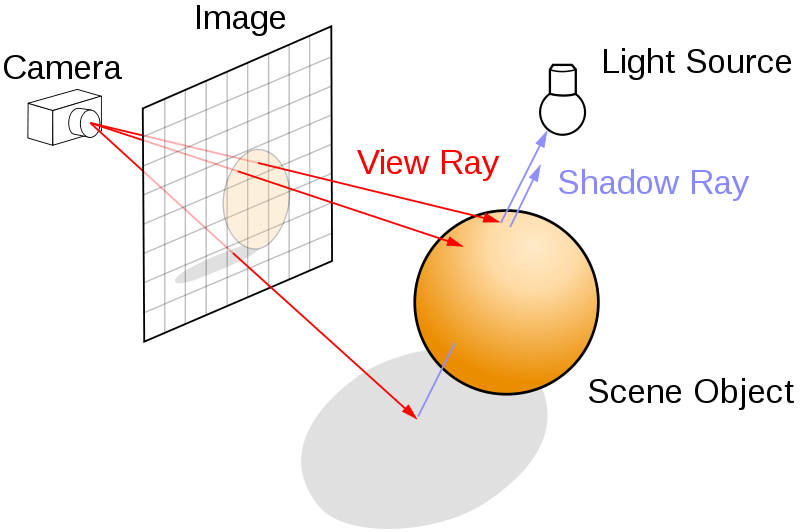
\includegraphics[scale=0.4]{res/ray_tracing.png}
\end{figure}

选定视点位置及一观察屏,从视点到屏上各点发出光线与空间中物体求交.
在交点处根据局部光照模型计算颜色,再递归的计算反射、透射光颜色,混合后显示在屏上.

